%-------------------------------------------------------------------------------

% This file is part of Code_Saturne, a general-purpose CFD tool.
%
% Copyright (C) 1998-2011 EDF S.A.
%
% This program is free software; you can redistribute it and/or modify it under
% the terms of the GNU General Public License as published by the Free Software
% Foundation; either version 2 of the License, or (at your option) any later
% version.
%
% This program is distributed in the hope that it will be useful, but WITHOUT
% ANY WARRANTY; without even the implied warranty of MERCHANTABILITY or FITNESS
% FOR A PARTICULAR PURPOSE.  See the GNU General Public License for more
% details.
%
% You should have received a copy of the GNU General Public License along with
% this program; if not, write to the Free Software Foundation, Inc., 51 Franklin
% Street, Fifth Floor, Boston, MA 02110-1301, USA.

%-------------------------------------------------------------------------------

\section{SOLUTION FOR CASE 5}
The preparation of the calculation for case 5 is very similar to the other cases.
\begin{itemize}
        \item Open the \CS interface
        \item Open a new case
        \item Check the name of the mesh
        \item Select a k-$\varepsilon$ model
        \item Use a thermal scalar in Celsius degrees
\end{itemize}

In the item {\itshape Initialization} under the heading {\itshape Volume conditions}, set the initial value of the temperature
in the domain to 38.5\degresC. Initialize the turbulence with the reference
velocity $0.03183\ m.s^{-1}$.

\begin{figure}[h!]
\begin{center}
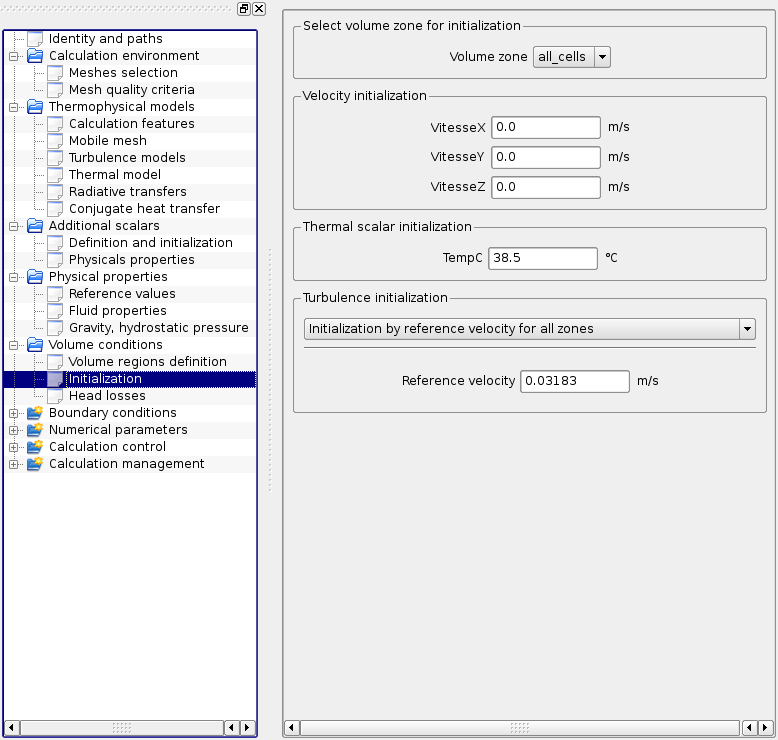
\includegraphics[width=12cm]{V-68}
\caption{Thermophysical models - Initialization}
\label{fig1_e5}
\end{center}
\end{figure}


\newpage
In the item {\itshape Fluid properties}, under the heading {\itshape Physical
properties}, enter the following information:

\begin{center}
\begin{tabular}{c|c|c}
Variable & Type & Value \\
\hline
Density & user law & $998.671\ kg.m^{-3} $ \\
\hline
Viscosity & user law & $0.445\times 10^{-4}\ kg.m^{-1}.s^{-1} $ \\
\hline
Specific Heat & Constant & $4\,182.88\ J.kg^{-1}.\mbox{\degresC}^{-1} $ \\
\hline
Thermal Conductivity & Constant & $0.601498\ W.m^{-1}.K^{-1}$
\end{tabular}
\end{center}

For density and viscosity, the value given here will serve as a reference
value (see user manual for details).

\begin{figure}[h!]
\begin{center}
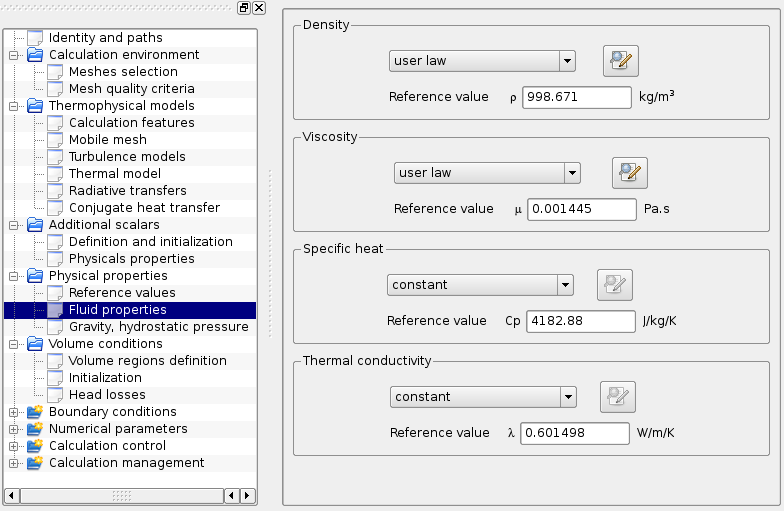
\includegraphics[width=12cm]{V-69}
\caption{Physical properties: fluid properties}
\label{fig2_e5}
\end{center}
\end{figure}

\newpage
For the density and viscosity, enter the expressions of the user laws as showed in
figures \ref{fig5_var1} and \ref{fig5_var2}, in the windows poping while clicking on the highlighted boxes.

\begin{figure}[h!]
\begin{center}
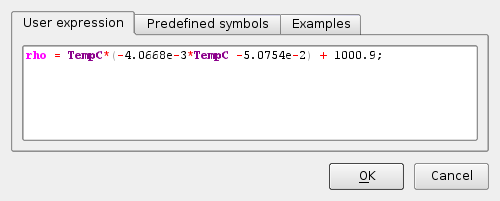
\includegraphics[width=12cm]{density_law}
\caption{Variable density}
\label{fig5_var1}
\end{center}
\end{figure}

\begin{figure}[h!]
\begin{center}
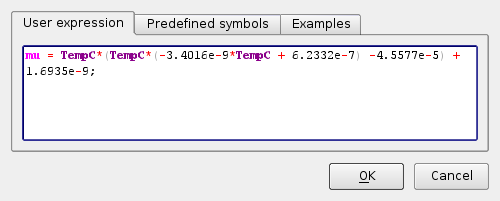
\includegraphics[width=12cm]{viscosity_law}
\caption{Variable viscosity}
\label{fig5_var2}
\end{center}
\end{figure}

\newpage
The aim of the calculation is to simulate a stratified flow. It is therefore
necessary to have gravity. Set it to the right value in the item
{\itshape Gravity, hydrostatic pressure}.  In order to have a sharper
stratification, the pressure interpolation method will be set to
{\itshape improved}.

\begin{figure}[h!]
\begin{center}
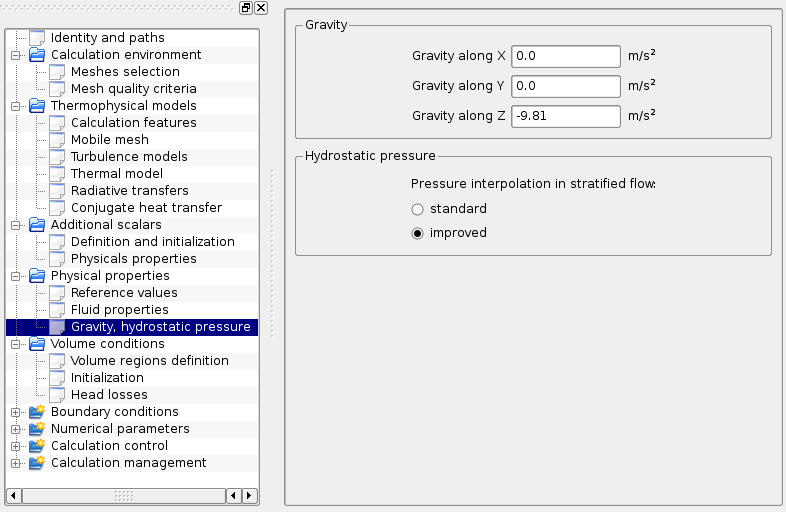
\includegraphics[width=12cm]{V-70}
\caption{Fluid properties - Gravity}
\label{fig3_e5}
\end{center}
\end{figure}


\newpage

Go to the item {\itshape Definition and initialization} under the heading
{\itshape Additional scalars} to specify the minimal and maximal values for the
temperature: 18.26\degresC\ and 38.5\degresC. Note that the initial value of
38.5\degresC\ set earlier is properly taken into account.

\begin{figure}[h!]
\begin{center}
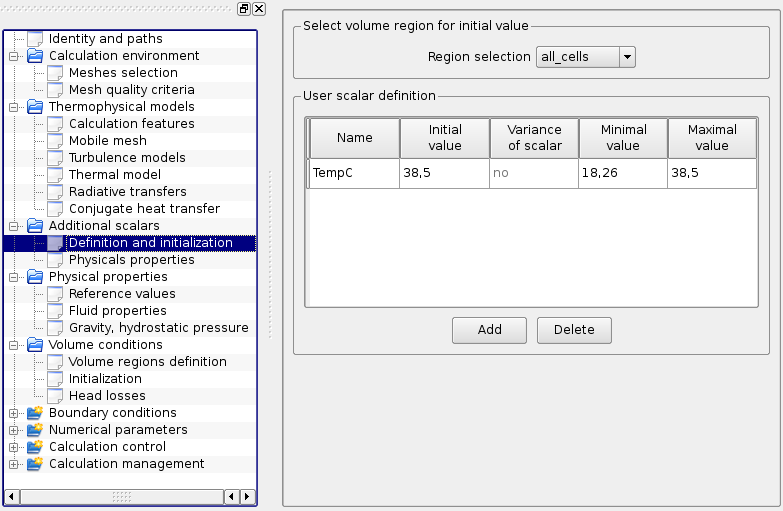
\includegraphics[width=12cm]{V-71}
\caption{Scalar initialization}
\label{fig4_e5}
\end{center}
\end{figure}


\newpage
Create the boundary regions.

\begin{center}
\begin{tabular}{|c|c|}
\hline
Colors & Conditions \\
\hline
2 & inlet \\
\hline
6 & inlet \\
\hline
7 & outlet \\
\hline
5 & wall \\
\hline
\end{tabular}
\end{center}

\begin{figure}[h!]
\begin{center}
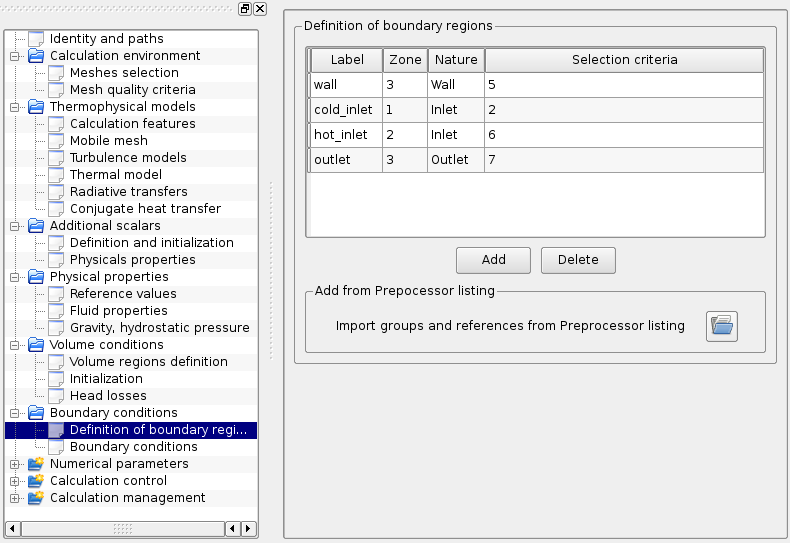
\includegraphics[width=12cm]{V-72}
\caption{Boundary regions}
\label{fig5_e5}
\end{center}
\end{figure}


\newpage
For the dynamic boundary conditions, the velocity is $0.03183\ m.s^{-1}$ in the
$z$ direction and the hydraulic diameter $0.4\ m$ for both inlets.


\begin{figure}[h!]
\begin{center}
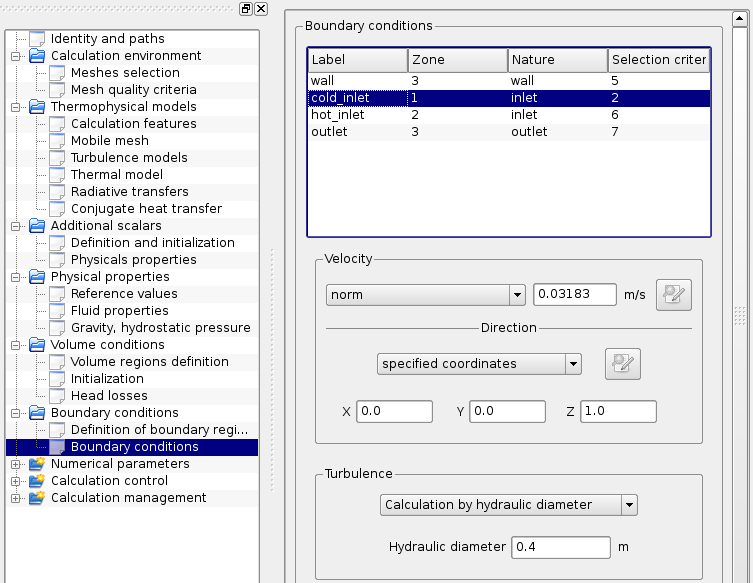
\includegraphics[width=12cm]{V-73}
\caption{Dynamic boundary conditions}
\label{fig6_e5}
\end{center}
\end{figure}

\begin{figure}[h!]
\begin{center}
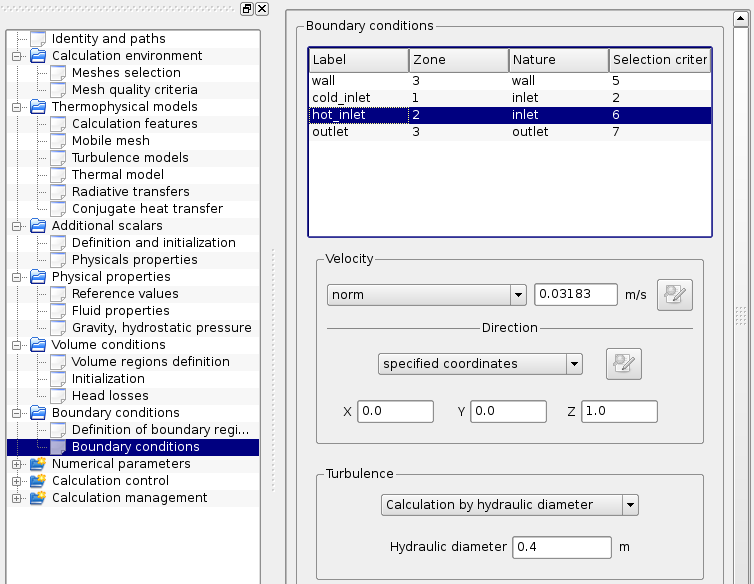
\includegraphics[width=12cm]{V-73bis}
\caption{Dynamic boundary conditions}
\label{fig6_e5}
\end{center}
\end{figure}

\newpage
For the scalar boundary conditions, the temperature of the cold inlet is
18.6\degresC\ and that of the hot inlet is 38.5\degresC.

\begin{figure}[h!]
\begin{center}
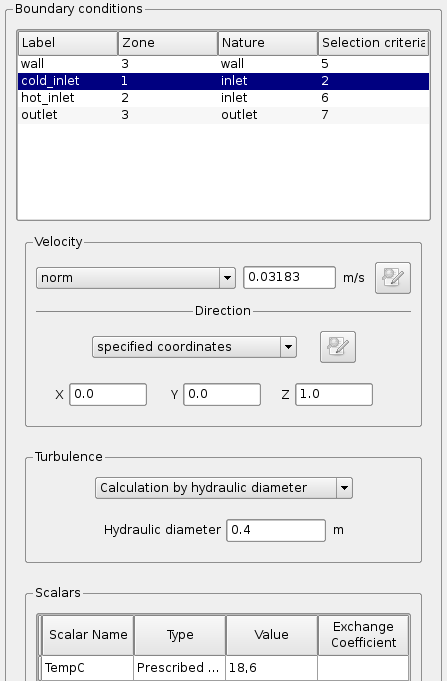
\includegraphics[width=8cm]{V-74}
\caption{Temperature boundary conditions}
\label{fig8_e5}
\end{center}
\end{figure}

\begin{figure}[h!]
\begin{center}
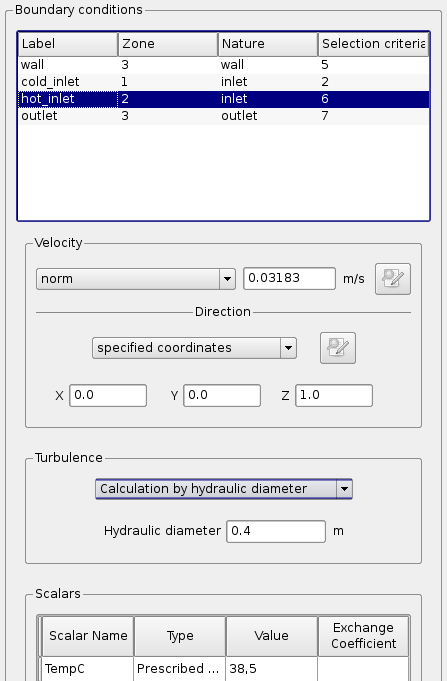
\includegraphics[width=8cm]{V-74bis}
\caption{Temperature boundary conditions}
\label{fig8_e5}
\end{center}
\end{figure}

\newpage
Tick the appropriate box for the time step to be variable in time and uniform in
space. In the boxes below, enter the following parameters:
\begin{center}
\begin{tabular}{|l|c|}
\hline
\multicolumn{2}{|c|}{Parameters of calculation control} \\
\hline
Number of iterations & 100 \\
\hline
Reference time step & $1\ s$ \\
\hline
Maximal CFL number & 20 \\
\hline
Maximal Fourier number & 60 \\
\hline
Minimal time step & $0.01\ s$ \\
\hline
Maximal time step & $70\ s$ \\
\hline
Time step maximal variation & $0.1$ \\
\hline
\end{tabular}\\
\end{center}

And activate the option
{\itshape Time step limitation with the local thermal time step}

\begin{figure}[h!]
\begin{center}
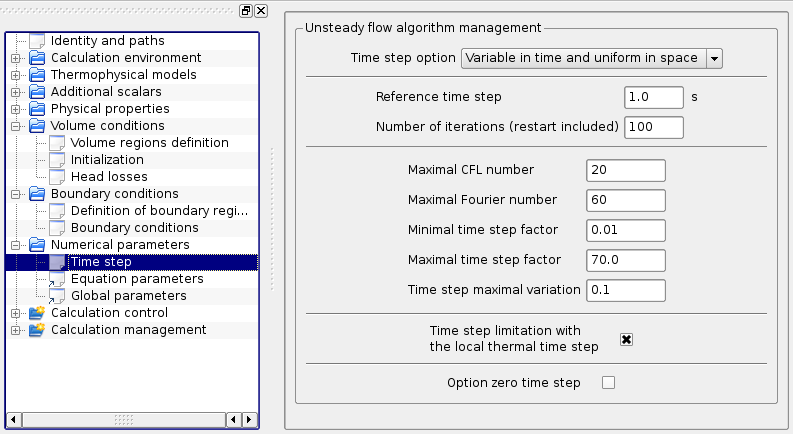
\includegraphics[width=13cm]{V-75}
\caption{Time step}
\label{fig11_e5}
\end{center}
\end{figure}


\newpage
Set the frequency of post-processing files to 10.

Create four monitoring probes at the following coordinates:
\begin{center}
\begin{tabular}{|c|c|c|c|}
\hline
Points & X(m) & Y(m) & Z(m)\\
\hline
1 & 0.010025 & 0.01534 & -0.011765 \\
\hline
2 & 1.625 & 0.01534 & -0.031652 \\
\hline
3 & 3.225 & 0.01534 & -0.031652 \\
\hline
4 & 3.8726 & 0.047481 & 7.25 \\
\hline
\end{tabular}
\end{center}

\begin{figure}[h!]
\begin{center}
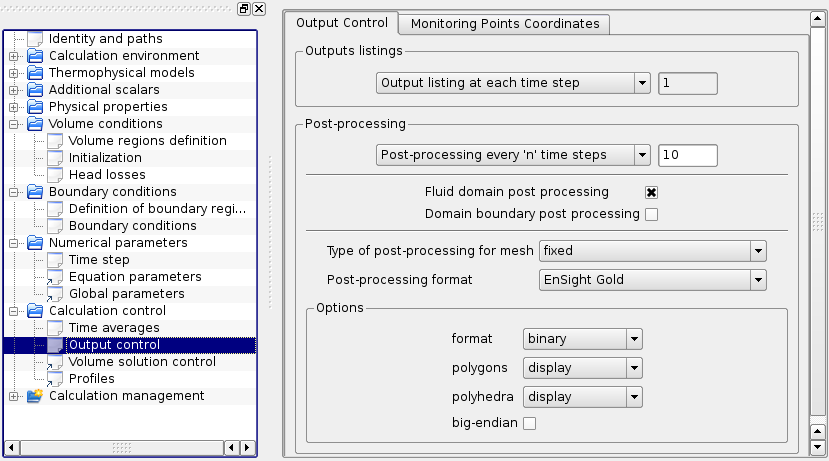
\includegraphics[width=12cm]{V-76}
\caption{Output management}
\label{fig12_e5}
\end{center}
\end{figure}

\begin{figure}[h!]
\begin{center}
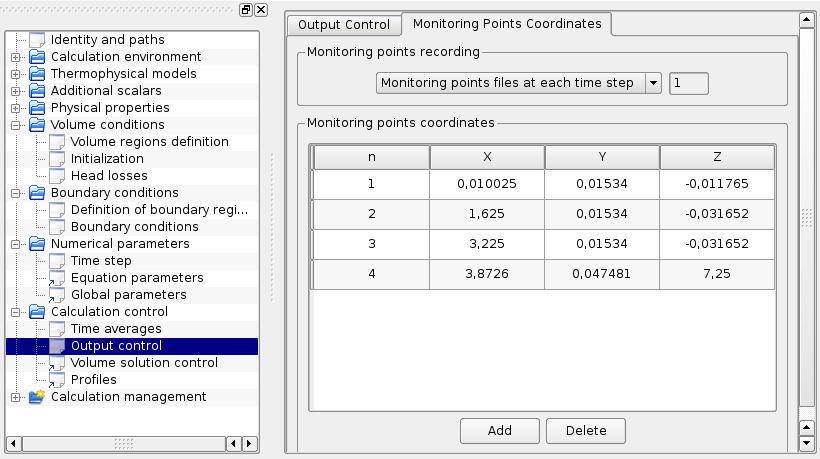
\includegraphics[width=12cm]{V-76bis}
\caption{Monitoring points}
\label{fig12bis_e5}
\end{center}
\end{figure}

\newpage
For the advanced post-processing features, copy the three routines
{\itshape usdpst.f90}, {\itshape usmpst.f90} and {\itshape usvpst.f90} in the SRC
directory. The general content of these routines is described in the user manual
or in the examples available in the directory SRC/REFERENCE/base. The modified
routines adapted to this test case are available in the \texttt{examples}
directory. Only the main elements are mentionned here.



$\bullet$ {\bfseries usdpst.f90}\\
This routine is called only once, at the beginning of the calculation. It allows
to define the different writers and parts.

The first writer is the standard writer (which creates the directory
CHR.ENSIGHT.xxxxxxxx). It is created by default and has the number -1.

Set the number of additional writers NBCAS to 1. For the first (and unique)
additional writer, specify the following elements :\\
\begin{tabular}{@{$\bullet\ $}l@{$\quad$}p{10cm}}
NOMCAS = 'chr' & prefix of the EnSight files\\
NOMREP = 'Tinf21.ensight' & name of the directory\\
NOMFMT = 'EnSight Gold' & format of the post-processing\\
OPTFMT = 'binary' & format options (here binary files)\\
INDMOD = 2 & indicates that the parts in this writer will be time dependent in its content\\
NTCHRL = 5 & periodicity of output\\
\end{tabular}
A directory TINF21.ENSIGHT.xxxxxxxx will be created with the post-processing
results associated to this writer.

Set the number of additional parts NBPART to 2.\\
For each part, set the number of cells, internal faces and boundary faces
(respectively NLCEL, NLFAC, NLFBR) and the lists LSTCEL, LSTFAC and LSTFBR of
the elements in the part\footnote{parts can only contain similar elements,
{\em i.e.} combinations of internal and boundary faces are allowed, but
combinations of cells and faces are not}.\\
The first part, the clip plane, will be created by detecting the internal faces
which have a center of gravity (CDGFAC) between -0.01 and 0.01.\\
The second part, the cells where the temperature is lower than 21\degresC, will
be specified in {\itshape usmpst.f90}. Yet it must be initialized in
{\itshape usdpst.f90}. The easiest is to set \mbox{NLCEL=NCEL}, total number of
cells (and when doing so, there is no need to specify the LSTCEL array).

Eventually, the different parts must be associated with the different writers,
through the PSTASS routine. Part 1 is associated to the writer -1, and part 2 to
the writer 1.


$\bullet$ {\bfseries usmpst.f90}\\
This routine is called at each time step. It allows to redefine the content of
certain parts using any variable, especially the temperature for this case.

Only part 2 is concerned. A DO/ENDDO loop on all the cells allows to identify those
where the temperature is lower than 21\degresC\ and hence calculate the number
of cells NCELPS in the part and the list of cells LSTCEL.


$\bullet$ {\bfseries usvpst.f90}\\
This routine is called at each time step. It allows to specify which variable
will be written on which part.

The writing in the post-processing files is triggered by the routine PSTEVA,
that must be called for each part and each variable to write. The arguments for
PSTEVA are:

\begin{tabular}{@{$\bullet\ $}l@{$\quad$}p{10cm}}
IPART & part number\\
NAMEVR & character string of the name under which the variable will be written\\
IDIMT & dimension of the variable (1 or 3 for scalars or vectors)\\
IENTLA & for vectors, indicates if the components are interlaced (=1) or not
(=0)\\
IVARPR & shortcut option for specific situations, set to 0 here\\
NTCABS & current time step (passed to {\itshape usvpst.f90} with the right value)\\
TTCABS & current physical time (passed to {\itshape usvpst.f90} with the right
value)\\
TRACEL & array for variables on cells\\
TRAFAC & array for variables on internal faces\\
TRAFBR & array for boundary faces
\end{tabular}


Part 1 only contains internal faces, so only TRAFAC needs to be filled. Execute
a loop on all the faces from the LSTFAC list. For each of them, the temperature
will be stored in TRAFAC.\\
The temperature at each face will be calculated by interpolation from the value
at the centers of the two neighboring cells. The numbers of the neighbors of
face IFAC are \mbox{IFACEL(IFAC,1)} and \mbox{IFACEL(IFAC,2)}. For a proper
linear interpolation, see in the TEST\_CASES directory for the use of the POND
parameter, yielding the fractionnal position of the face on the line joining the
two cell centers.\\
Note that in parallel computing, the cells on both side of the face can be
managed by different processors. In order for the interpolation to be correct, a
parallel synchronization must be done before the loop. A similar problem happens
with periodic boundary conditions. Hence the calling of routines PARCOM and
PERCOM shown in the example in the TEST\_CASES directory.

As for part 2, it contains only cells so only TRACEL need be filled. For each
cell in the LSTCEL list, just set TRACEL to the value of the temperature at the
center of the cell.
